%version of 08-07-19
\chapter{The Diverse Delights of de Bruijn Networks}
\label{ch:de-Bruijn-delights}

\section{Cycles in de Bruijn Networks}
\label{Appendix:deBruijn-Hamiltonian}

This section is devoted to proving Proposition~\ref{thm:deBruijn-Hamiltonian}:

\noindent
{\em
For all $n \in \N^+$, $\d_n$ contains a {\em directed Hamiltonian
  cycle}, i.e., a length-$2^n$ directed cycle of the form
\[
 x \ \rightarrow \ y_1 \ \rightarrow \ y_2 \ \rightarrow \cdots
\ \rightarrow \ y_{2^n-1} \ \rightarrow \ x
\]
which contains every node of $\d_n$ precisely once; i.e.:
\begin{itemize}
\item
$\{x, \ y_1, \ y_2, \ldots, \ y_{2^n-1}\} \ = \ \n_{\fd_n}$.
\item
All of the ``$y$-nodes'' that appear in cycle
(\ref{eq:deBruijn-cycle}) differ from $x$ and from each other.
\end{itemize}
}

The simplest proof of this result has two steps.  We now begin to develop these concepts and the proof.

\bigskip

\noindent {\bf (1)}
%
For any directed graph $\g$, the {\it line digraph} \index{line graph}
\index{line digraph} of $\g$, denoted $\Lambda(\g)$, is the following
directed graph.
\begin{itemize}
\item
The nodes of $\Lambda(\g)$ are the arcs of $\g$:
\[ \n_{{\Lambda}({\cal G})} \ = \ \a_{\fg} \]
\item
For each pair of arcs of $\g$ of the form
\[ \big[a_{x,y} = (x \ \rightarrow \ y) \big] \ \ \ \mbox{ and } \ \ \ 
\big[a_{y,z} = (y \ \rightarrow \ z) \big]
\]
i.e, arcs such that the endpoint of the first arc is the source of the
second arc, $\Lambda(\g)$ contains an arc $(a_{x,y} \ \rightarrow
\ a_{y,z})$.
\end{itemize}
The relevance of this topic to this section is that the line graph of
every de Bruijn network $\d_n$ is the ``next bigger'' de Bruijn
network, $\d_{n+1}$.  Let us verify this claim.

\begin{prop}
\label{thm:deBruin-linegraph}
For all $n \in \N^+$,
$\d_{n+1}$ is the line digraph of $\d_n$: $\d_{n+1} \ = \ \Lambda(\d_n)$.
\end{prop}


\begin{proof}
Each node of $\Lambda(\d_n)$ is an arc of $\d_n$, hence has the form
\[ (\beta x \ \rightarrow \ x \gamma) \]
for $x$ a length-$(n-1)$ binary string and $\beta, \gamma \in
\{0,1\}$.  Let us associate node $\beta x \gamma$ of $\d_{n+1}$ with
this node of $\Lambda(\d_n)$.

\smallskip

Note first that each arc of $\d_{n+1}$ has the form
\[ (\delta y \varepsilon \ \rightarrow \ y \varepsilon \varphi), \]
where $y$ is a length-$(n-2)$ binary string and $\delta, \varepsilon,
\varphi \in \{0,1\}$.  By our association of nodes of $\d_{n+1}$ with
arcs of $\d_n$, this arc of $\d_{n+1}$ does, indeed, correspond to two
successive arcs of $\d_n$.   The first of these successive arcs
{\em enters} node $y \varepsilon$ of $\d_n$; the second {\em leaves}
that node.


Note next that, given any two successive arcs of $\d_n$, say
\[
(\rho \sigma z \ \rightarrow \ \sigma z \tau) \ \ \ \mbox { and } \ \ \
(\sigma z \tau \ \rightarrow \  z \tau \xi)
\]
where $z$ is a length-$(n-2)$ binary string and $\rho, \sigma, \tau,
\xi \in \{0,1\}$, there is, indeed, an arc of $\d_{n+1}$ of the form
\[ (\rho \sigma z \tau \ \rightarrow \ \sigma z \tau \xi) \]
This means that the digraph $\d_{n+1}$ is identical to the digraph
$\Lambda(\d_n)$, modulo a renaming of nodes and arcs.\footnote{Technically,
  we are asserting that the digraphs ${\cal D}_{n+1}$ and ${\Lambda}({\cal D}_n)$ 
  are {\it isomorphic} to one another.  The topic of
  graph isomorphism is beyond the scope of this text, but our informal
  description provides all the details one would need to formalize the
  described isomorphism.}

The described correspondence between the nodes and arcs of $\d_{n+1}$
and $\Lambda(\d_n)$ completes the proof.  \qed
\end{proof}

\begin{figure}[hbt]
\begin{center}
       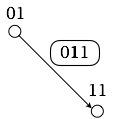
\includegraphics[scale=0.6]{FiguresGraph/dBlabelEdge}
\caption{Illustrating how to label each arc of a de Bruijn network by
  concatenating the labels of the nodes incident to the arc and
  compacting the common intermediate bits.  In the depicted example,
  the node-labels $01$ and $11$ combine to yield the arc-label $011$.}
  \label{fig:dBlabelEdge-App}
\end{center}
\end{figure}

\medskip

\noindent {\bf (2)}
{\it Eulerian cycles (or tours)}. \index{Eulerian cycle}
\index{Eulerian tour} A {\it directed Eulerian cycle} in a digraph
$\g$ is a directed cycle that contains each arc of $\g$ precisely
once.  We will see, later in this chapter, a truly elementary
argument, based on node-degrees, which proves that every de Bruijn
digraph has a directed Eulerian cycle.  This demonstration will
combine with Proposition~\ref{thm:deBruin-linegraph} to complete the
proof of Proposition~\ref{thm:deBruijn-Hamiltonian}.  \qed
%\end{proof}



\section{Connecting Trees with DeBruijn Networks via Algebra} 
\label{Appendix:tree-DB}




\[
\begin{array}{|ccccccc|}
\hline
\multicolumn{3}{c}{\mbox{Arc-labels: Tree}} & \hspace*{.2in}& \multicolumn{3}{c}{\mbox{Arc-labels: De Bruijn network}} \\
\hline 
F_0(x) & = & 2x      &  &  F^{(n)}_0(x) & = & 2x \bmod 2^n \\
F_1(x) & = & 2x+1  &  &  F^{(n)}_1(x) & = & 2x +1 \bmod 2^n \\ 
\hline
\end{array}
\]

\[
\begin{array}{|c|ccccc|}
\hline
\mbox{vertex} & \multicolumn{2}{c}{\mbox{Tree-successor}} & \hspace*{.2in} & \multicolumn{2}{c}{\mbox{DeBruijn-successor}} \\
\hline
v & F_0(v) & F_1(v) & & F^{(n)}_0(v))& F^{(n)}_1(v) \\
\hline
0 & 0 & 1 & & 0 & 1 \\ 
1 & 2 & 3 & & 2 & 3 \\
2 & 4 & 5 & & 4 & 5 \\
3 & 6 & 7 & & 6 & 7 \\
4 & \cdots & \cdots  & & 0 & 1 \\
5 & \cdots & \cdots  & & 2 & 3 \\
6 & \cdots & \cdots  & & 4 & 5 \\
7 & \cdots & \cdots  & & 6 & 7 \\
\hline
\end{array}
\]
